\chapter{Implementácia softvérovej časti}
\label{ImplementaciaSW}

Softvérová vrstva systému prepája centrálny backend na platforme
Raspberry~Pi s~periférnymi uzlami ESP32 a~nadväzuje na architektonický
návrh z~kapitoly~\ref{NavrhArchitektury} aj hardvérovú realizáciu
z~kapitoly~\ref{ImplementaciaHW}. Zabezpečuje vykonávanie scén,
koordináciu multimédií, odosielanie príkazov na fyzické zariadenia
a~vyhodnocovanie ich spätnej väzby.

\section{Softvérová architektúra systému}
\label{SWAchitektura}

Koncepčné dvojúrovňové rozdelenie z~kapitoly~\ref{NavrhArchitektury}
je v~tejto časti rozpracované do konkrétnych backendových
a~firmvérových komponentov pre beh scény.

Softvérová architektúra je navrhnutá ako trojica previazaných vrstiev,
pričom hlavným princípom je \textbf{separácia zodpovedností}:
backend neobsahuje hardvérovo špecifickú logiku GPIO výstupov
a~firmvér uzlov neobsahuje scenárové vetvenie expozície.
Vďaka tomu je možné upravovať scenáre, webové rozhranie
alebo firmvér uzla oddelene, zatiaľ čo tok informácií medzi vstupmi,
backendom, MQTT brokerom, uzlami ESP32 a~webovým dashboardom
ostáva vymedzený (Obr.~\ref{fig:sw_layers}).

\begin{figure}[H]
    \centering
    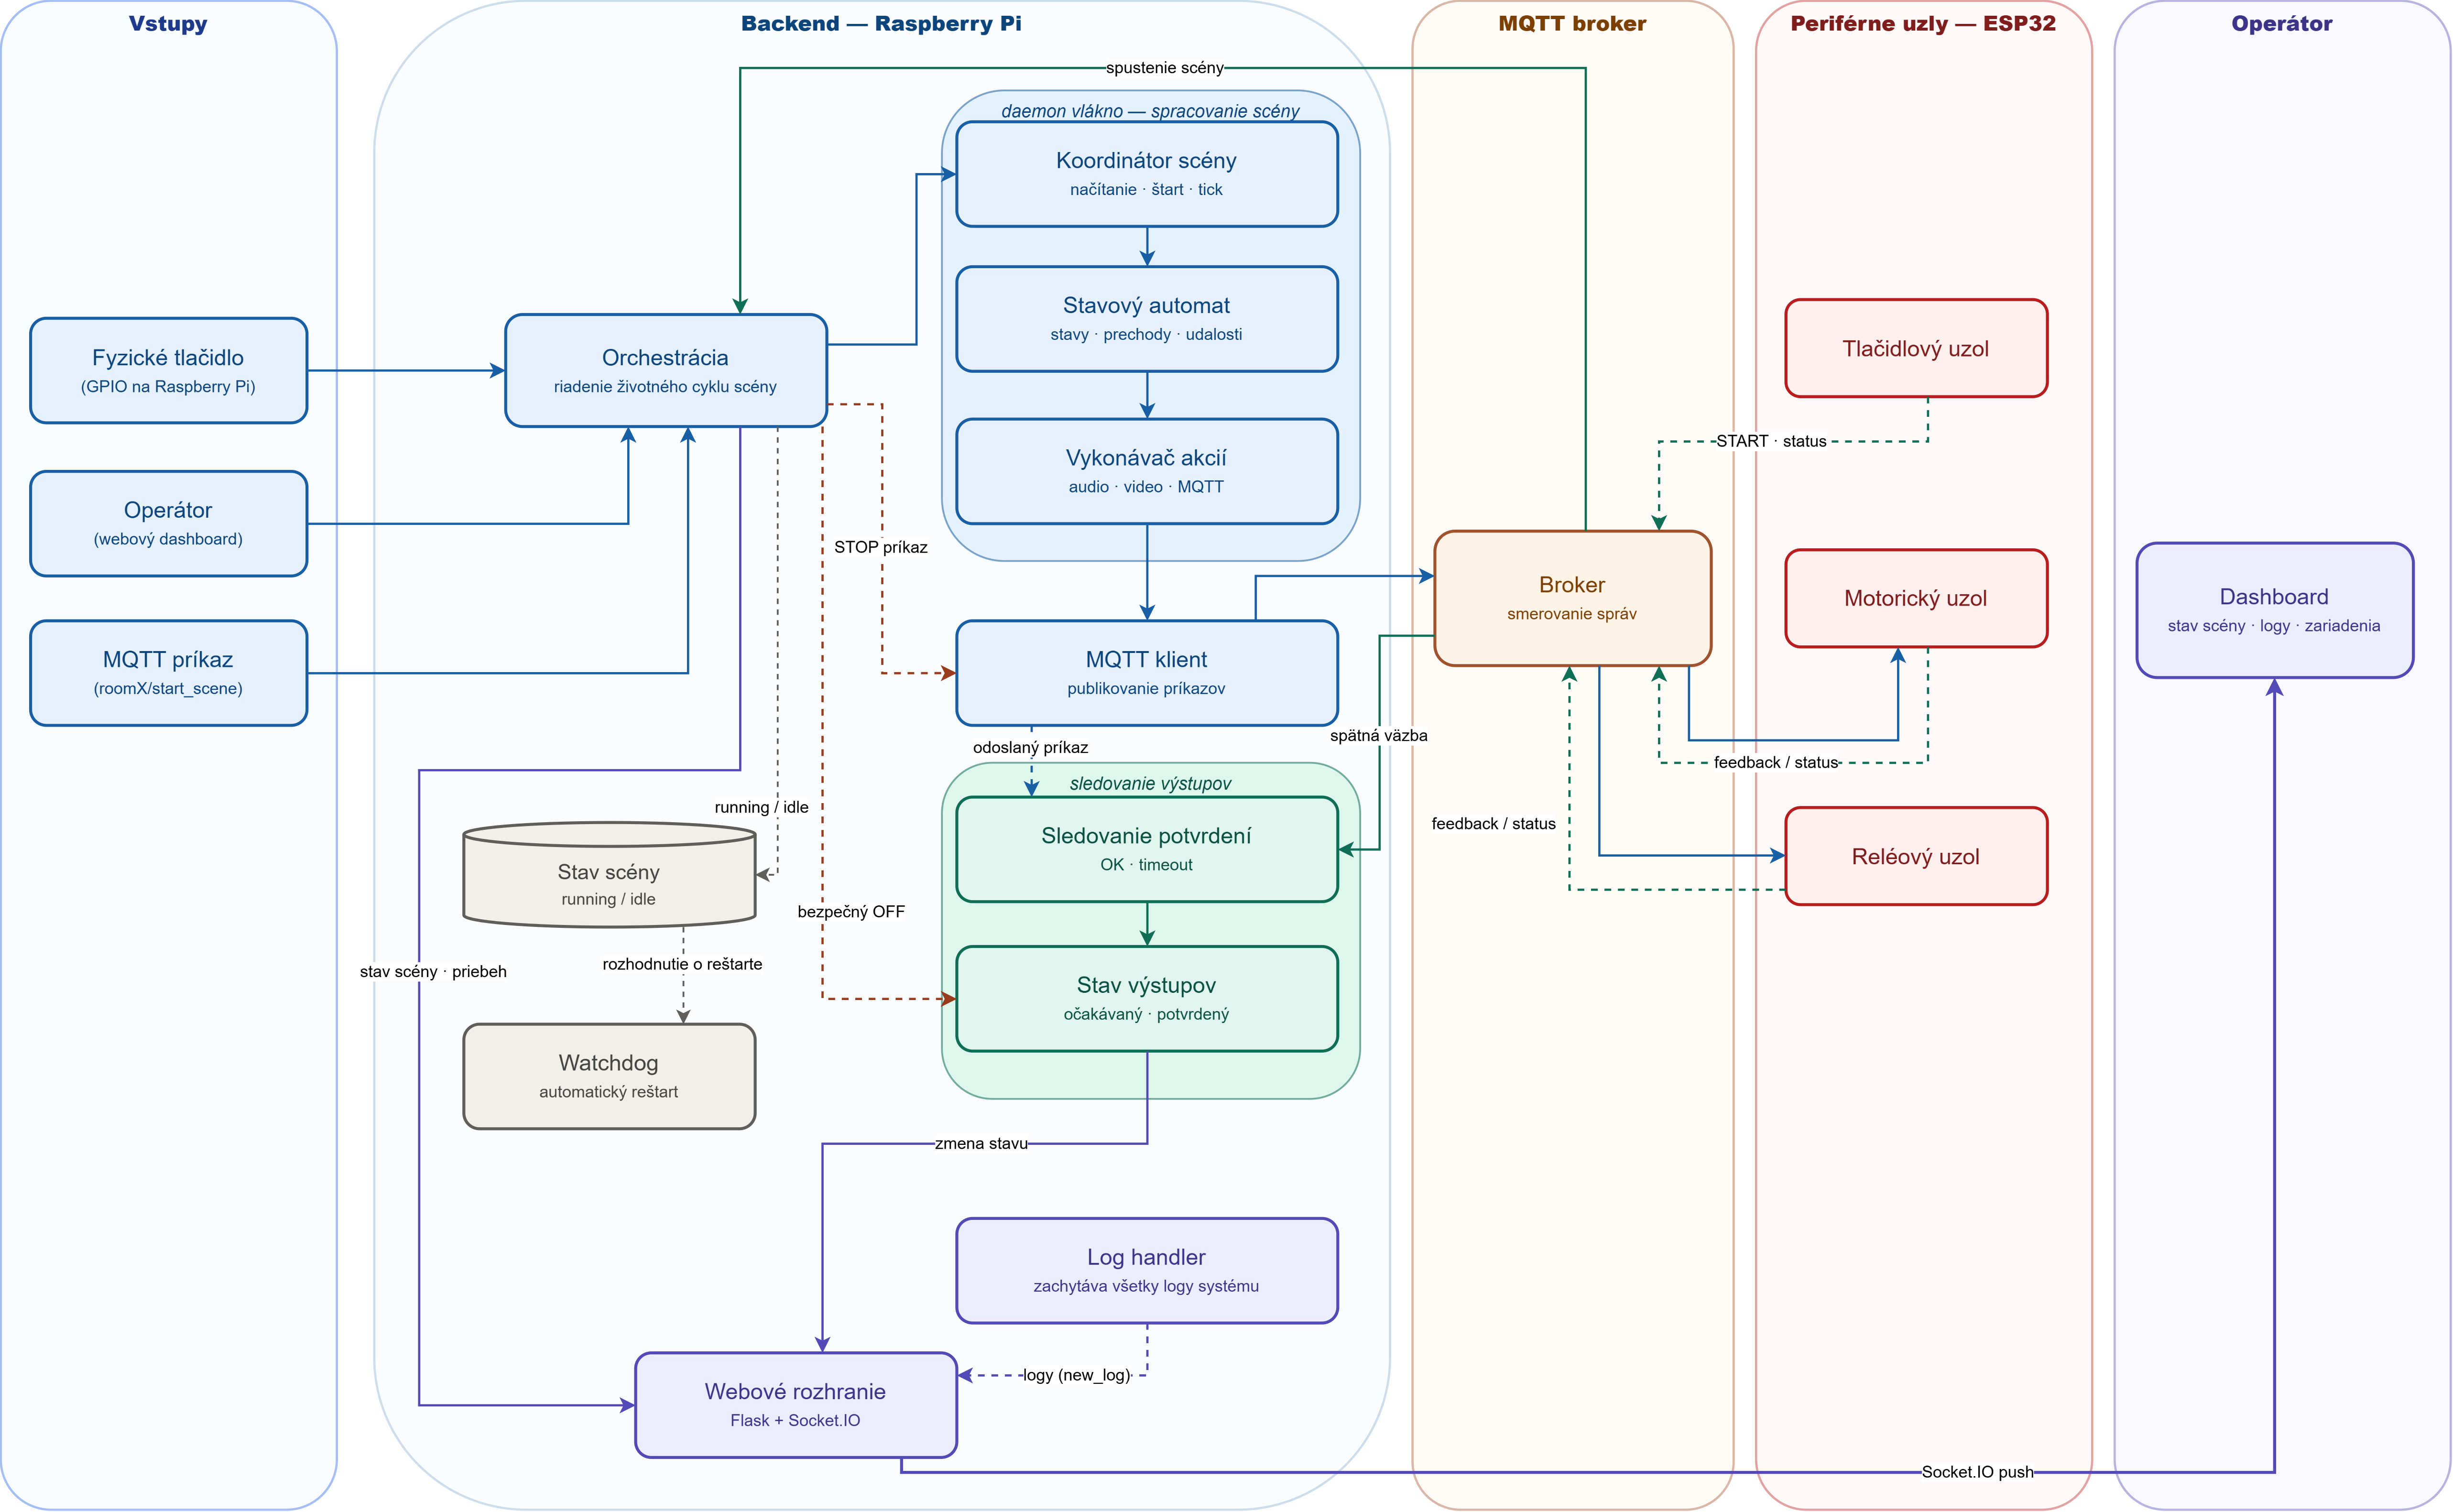
\includegraphics[width=1.00\linewidth,height=0.90\textheight,keepaspectratio]{obr/SW_DIAGRAM_SPECS/5_1_runtime_loop/diagram_5_1_runtime_loop_final.png}
    \caption{Softvérové vrstvy systému a~ich väzby}
    \label{fig:sw_layers}
\end{figure}

\section{Backend Raspberry~Pi}
\label{SWBackendRPI}

Backendová časť je implementovaná v~jazyku \textbf{Python} a~nasadená
ako systémová služba členená do šiestich funkčných celkov pokrývajúcich
celý životný cyklus behu scény (Obr.~\ref{fig:sw_backend_lifecycle}).

\begin{figure}[H]
    \centering
    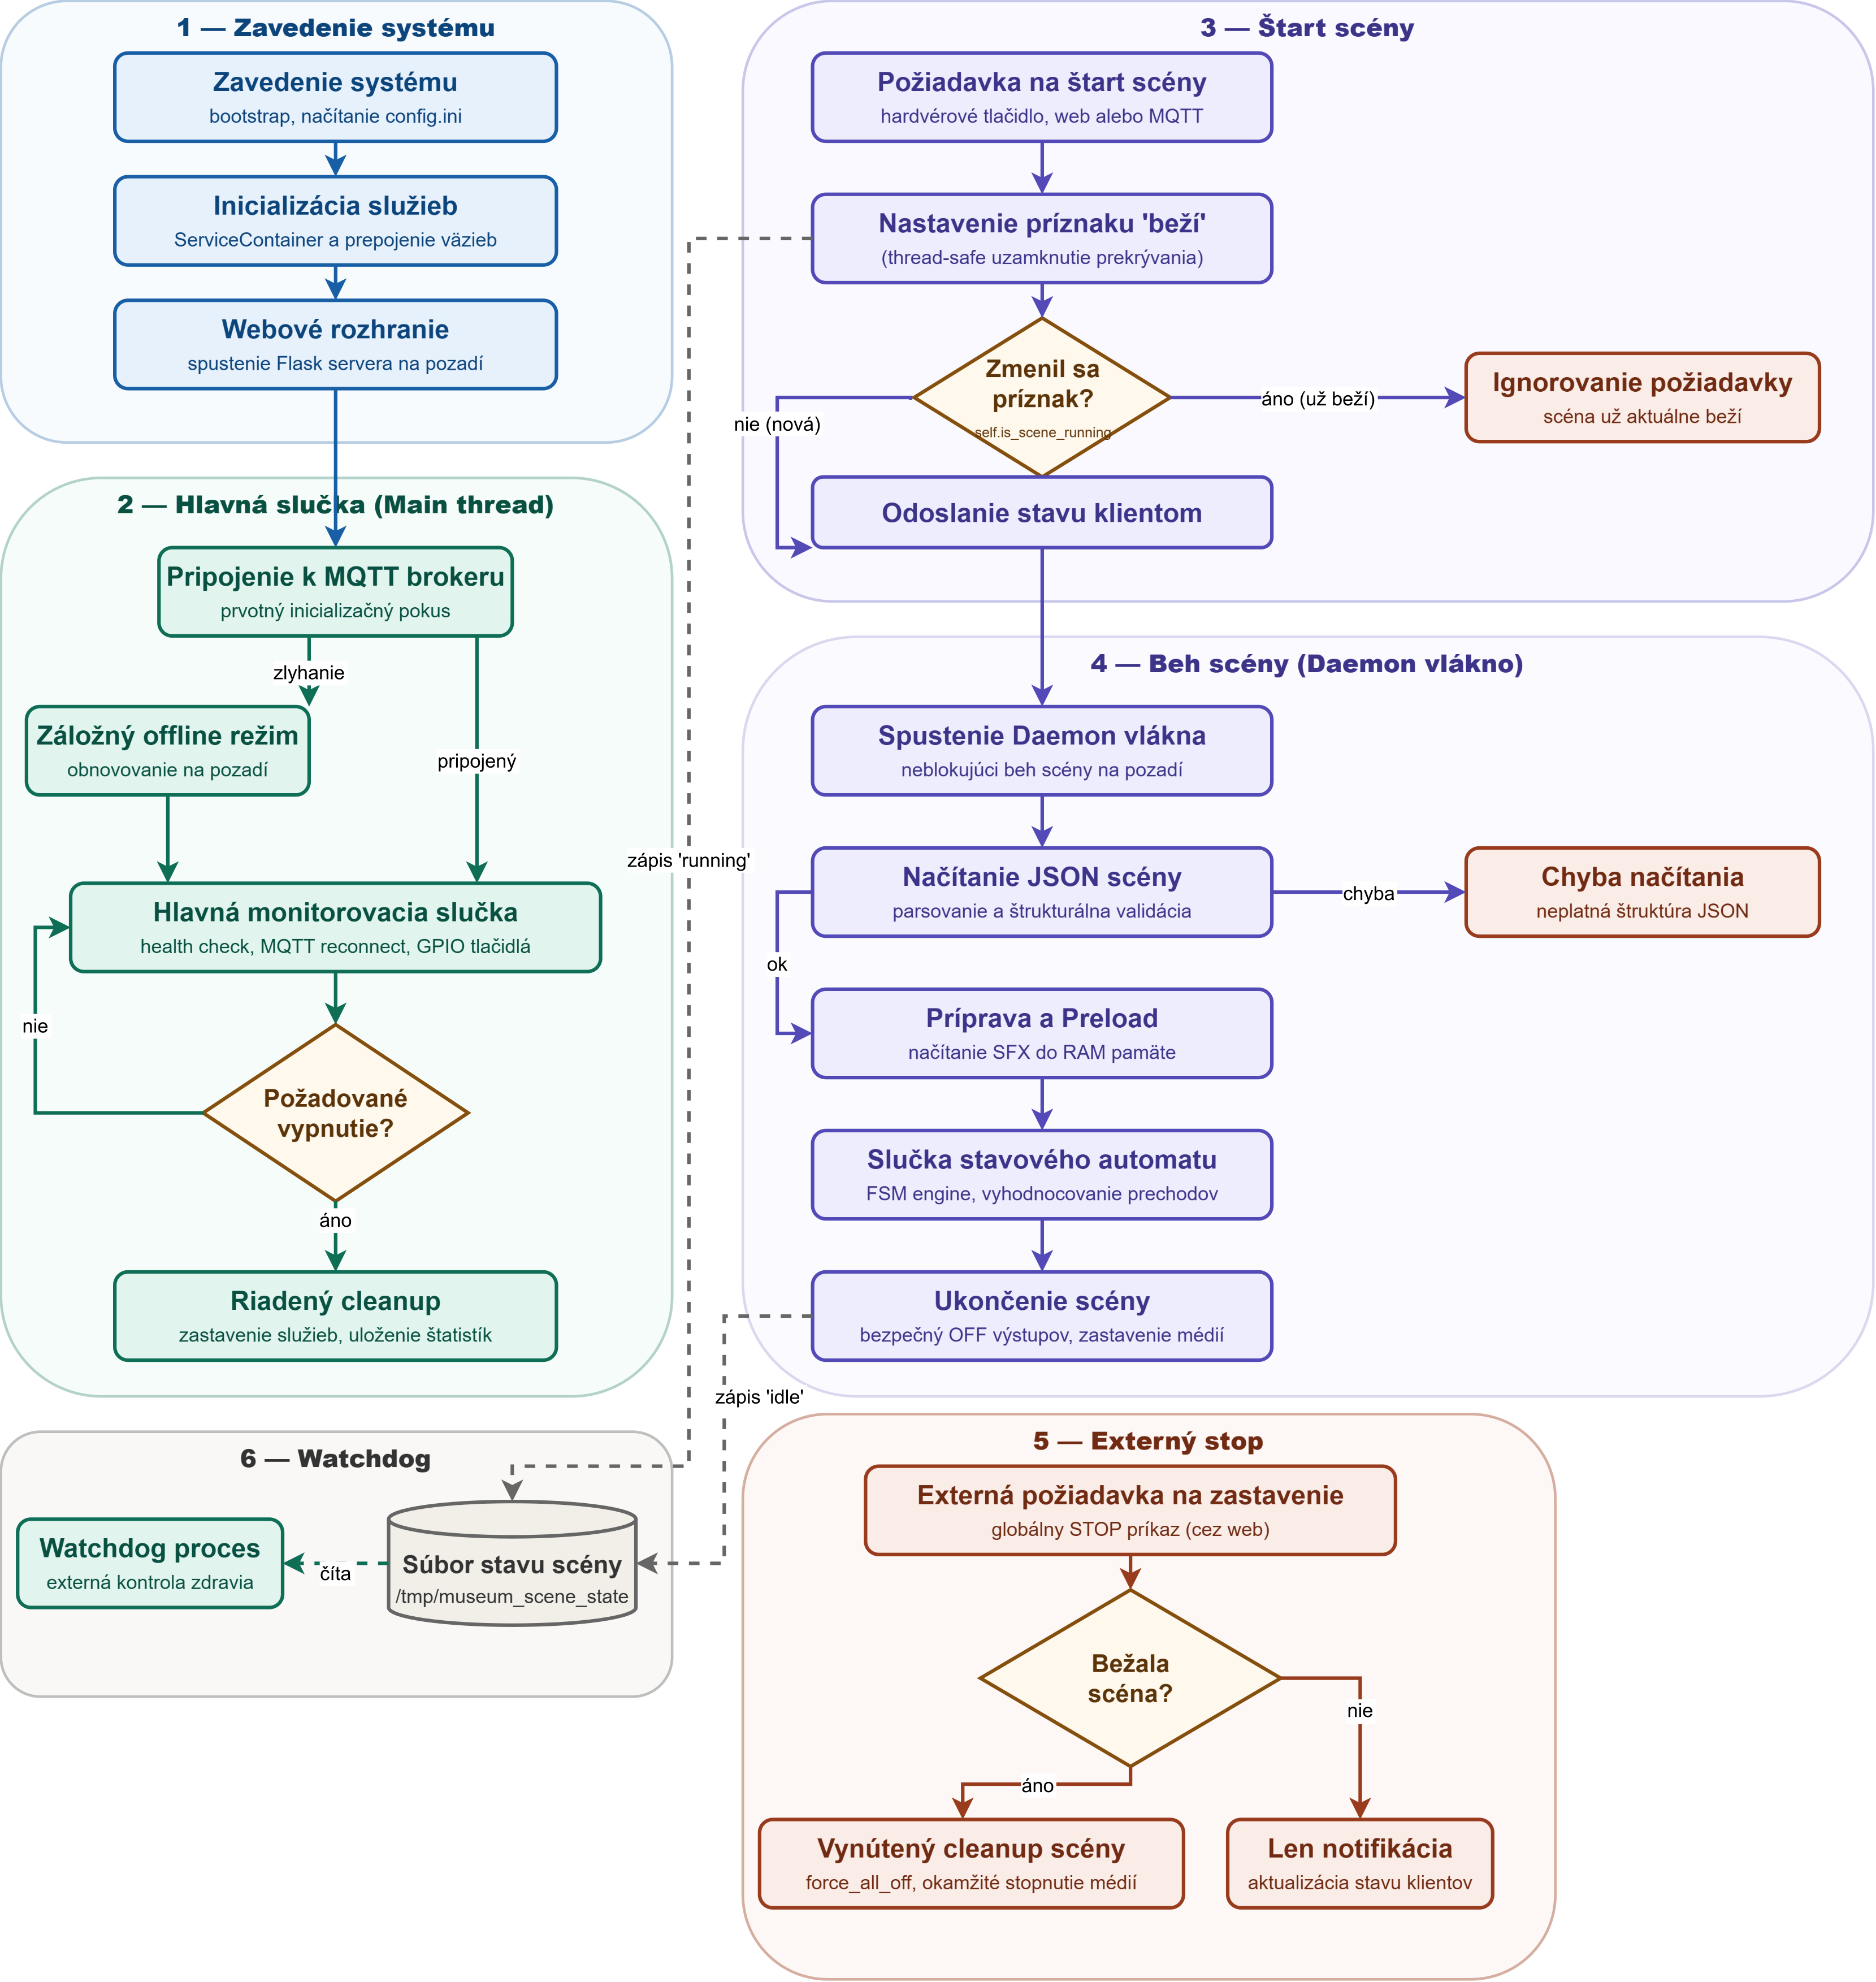
\includegraphics[width=0.95\linewidth,height=0.72\textheight,keepaspectratio]{obr/SW_DIAGRAM_SPECS/5_2_backend_lifecycle/diagram_5_2_backend_lifecycle_final.png}
    \caption{Životný cyklus backendovej služby}
    \label{fig:sw_backend_lifecycle}
\end{figure}

\subsection{Orchestrácia behu systému}
\label{SWOrchestracia}

Pri štarte backend načíta konfiguráciu z~inicializačného súboru
(MQTT parametre, GPIO vstupy, cesty k~médiám, identifikátor
miestnosti a~logovanie). Konfigurácia runtime je oddelená
od obsahovej konfigurácie scén.

Po načítaní konfigurácie backend inicializuje runtime služby,
prepojí ich callback mechanizmami a~spustí hlavnú slučku,
v~ktorej sa periodicky vyhodnocuje stav MQTT spojenia,
dostupnosť zariadení a~vstupy fyzického tlačidla. Samotné vykonávanie
scény prebieha v~separátnom \textbf{daemon vlákne}, takže hlavná slučka
nie je blokovaná počas behu scenára a~môže naďalej obsluhovať
periférne udalosti a~kontrolovať zdravie systému.

Pri ukončení systému sa vykoná \textbf{riadené ukončenie služby}
so zastavením aktívnej scény, vypnutím výstupov a~zaznamenaním
prevádzkových údajov. Tým sa znižuje riziko, že po ukončení služby
ostane časť zariadení v~neželanom stave.

\subsection{Watchdog a~odolnosť voči výpadkom}
\label{SWWatchdog}

Okrem hlavnej služby beží samostatná \textbf{watchdog služba},
ktorá monitoruje zdravie backendového procesu a~v~prípade poruchy
ho automaticky reštartuje. Pred reštartom kontroluje prevádzkový príznak
aktuálneho behu scény zapisovaný hlavnou službou do stavového súboru.
Ak je scéna aktívna, watchdog čaká na jej dokončenie v~periodických
intervaloch a~po prekročení pevného časového limitu pokračuje
reštartom, aby sa zabránilo nekonečnému čakaniu pri zlyhaní hlavného
procesu.

\subsection{Stavový automat ako jadro logiky}
\label{SWFSM}

Spracovanie scény je v~implementácii rozdelené na načítanie
a~validáciu konfiguračného súboru, evidenciu aktuálneho stavu,
vyhodnocovanie podmienok prechodov a~vykonávanie akcií. Poradie týchto
krokov v~jednom cykle behu scény je zhrnuté na
Obr.~\ref{fig:sw_fsm_engine}.

Podporované typy prechodov medzi stavmi sú:
\begin{itemize}
    \item \textbf{Časový limit} --- prechod po uplynutí nastaveného času,
    \item \textbf{Koniec audia} --- prechod po dohratí zvukovej stopy,
    \item \textbf{Koniec videa} --- prechod po dohratí videoklipu,
    \item \textbf{MQTT správa} --- prechod po prijatí správy od uzla (napr. stlačenie tlačidla),
    \item \textbf{Bezpodmienečný prechod} --- vykoná sa vždy pri vstupe do stavu.
\end{itemize}
Vyhodnocovanie prebieha v~poradí, v~akom sú prechody zapísané
v~konfiguračnom súbore; pri splnení prvej podmienky sa okamžite
vykoná príslušný prechod.

Okrem lokálnych prechodov sú podporené aj \textbf{globálne podmienky}
platné pre celú scénu bez ohľadu na aktuálny stav, najmä pre núdzové
zastavenie a~celkové časové limity. V~cykle behu scény majú
globálne podmienky prednosť pred lokálnou logikou jednotlivých stavov,
čím sa zabezpečuje,
že núdzové alebo celoscénové pravidlá ovplyvnia ďalší krok
ešte pred bežnými prechodmi stavu (Obr.~\ref{fig:sw_fsm_engine}).

Konkrétny priebeh expozície sa preto do vykonávacej logiky
vkladá prostredníctvom externej JSON konfigurácie opísanej
v~nasledujúcej podsekcii.

\begin{figure}[H]
    \centering
    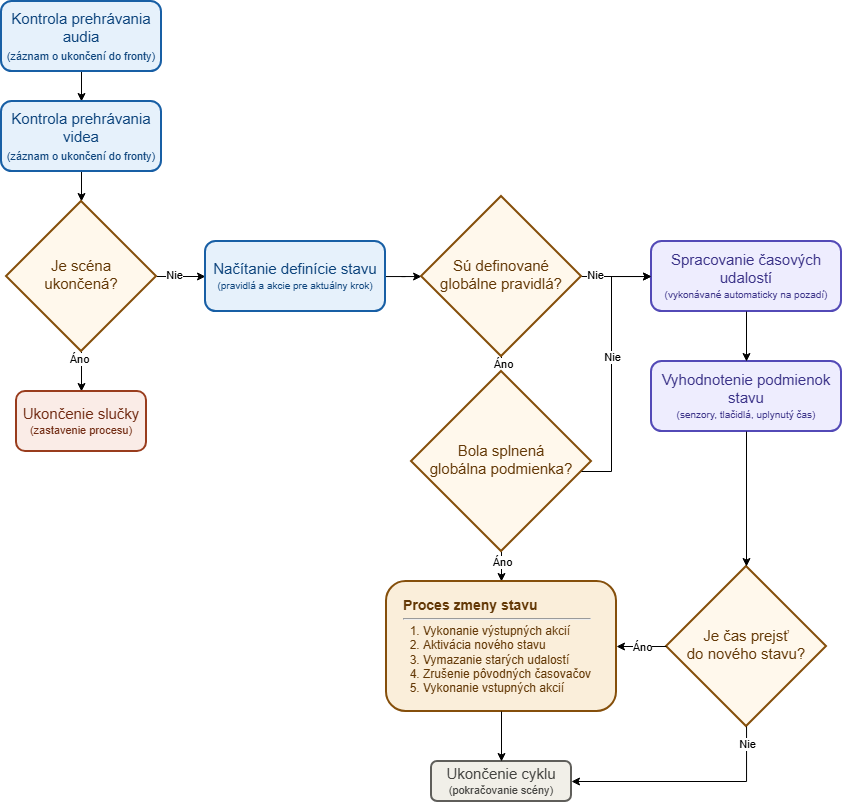
\includegraphics[width=0.95\linewidth,height=0.80\textheight,keepaspectratio]{obr/SW_DIAGRAM_SPECS/5_3_fsm_engine_tick_flow/diagram_5_3_fsm_engine_tick_flow_final.png}
    \caption{Poradie spracovania stavového automatu v~jednom cykle}
    \label{fig:sw_fsm_engine}
\end{figure}

\subsection{JSON konfigurácia ako vstup stavového automatu}
\label{SWJSON}

Návrh externej JSON konfigurácie uvedený v~kapitole~\ref{KomunikacnaVrstva}
je implementovaný ako množina samostatných súborov scén načítavaných
podľa požadovaného priebehu expozície. V~rámci jednej miestnosti
tak môže existovať viacero alternatívnych alebo testovacích scén,
pričom každá opisuje vlastnú postupnosť stavov, akcií a~prechodov.
Oddelenie scenára od enginu umožňuje meniť priebeh scény bez úprav
zdrojového kódu backendu.

Každá scéna obsahuje identifikátor, počiatočný stav
a~slovník stavov, pričom každý stav sa ďalej skladá zo sekcií
pre vstupné akcie, časovú os, výstupné akcie a~prechody
(Obr.~\ref{fig:sw_json_structure}).

Sekcia časovej osi umožňuje plánovať udalosti relatívne voči vstupu
do stavu bez blokovania zvyšku systému; v~implementácii sú tieto akcie
realizované ako asynchrónne časovače. Podporované akcie sú tri:
\textbf{MQTT akcia}, \textbf{audio akcia}
a~\textbf{video akcia}; ich príkazové formáty spolu s~tópikmi
na spustenie scény sú uvedené v~tom istom prehľade
(Obr.~\ref{fig:sw_json_structure}).

Pri zmene stavu sa plánovanie časovej osi resetuje, takže akcie
z~predchádzajúceho stavu nemôžu zasiahnuť do nového stavu.

Pred spustením scény prebieha \textbf{schémová a~logická validácia},
ktorá kontroluje povinné polia, typy a~existenciu cieľových stavov
prechodov. Tým sa eliminuje spúšťanie neplatných konfigurácií.

\begin{figure}[H]
    \centering
    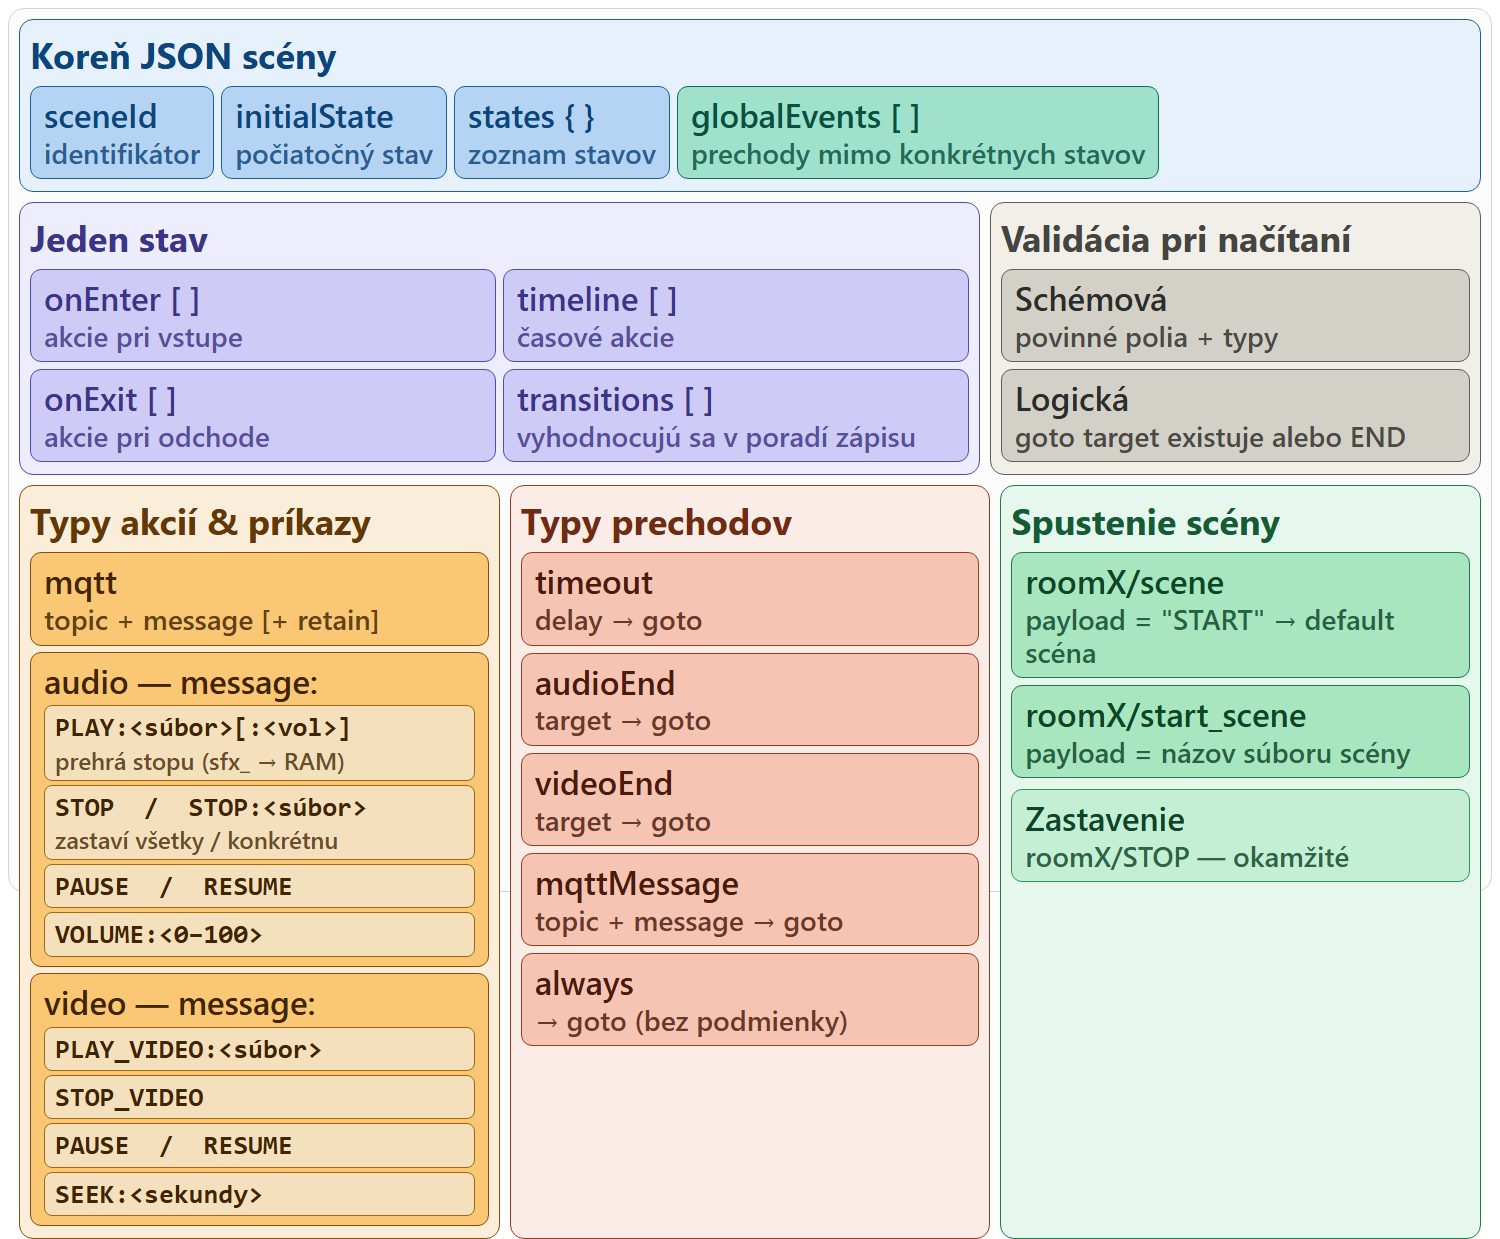
\includegraphics[width=0.92\linewidth,height=0.80\textheight,keepaspectratio]{obr/SW_DIAGRAM_SPECS/5_4_json_scene_structure/diagram_5_4_json_scene_structure_final_html.png}
    \caption{Štruktúra konfiguračnej scény}
    \label{fig:sw_json_structure}
\end{figure}

\section{MQTT komunikačná vrstva}
\label{SWMQTT}

Úlohu sieťového sprostredkovateľa správ zabezpečuje softvér
\textbf{Mosquitto}, spustený ako systémová služba priamo
na Raspberry~Pi. Broker používa port \textbf{1883}, cez ktorý
komunikuje Python backend s~uzlami ESP32.

Komunikačná vrstva zabezpečuje výmenu správ medzi backendom
a~uzlami ESP32. Po úspešnom pripojení backend odoberá stavové
topiky zariadení, topiky spätnej väzby a~miestnostné topiky určené
pre scénické udalosti alebo príkazy aktuátorom. Základné skupiny správ
sú rozdelené podľa účelu komunikácie (Tab.~\ref{tab:sw_mqtt_topics}).

\begin{table}[htbp]
    \centering
    \caption{Skupiny MQTT správ používané v~komunikačnej vrstve}
    \label{tab:sw_mqtt_topics}
    \small
    \begin{tabular}{|p{0.21\linewidth}|p{0.37\linewidth}|p{0.32\linewidth}|}
        \hline
        \textbf{Skupina správ} & \textbf{Topik} & \textbf{Smer a~účel} \\
        \hline
        Spustenie scény &
        \texttt{roomX/scene}, \texttt{roomX/start\_scene} &
        Vstup do backendu; spustenie predvolenej alebo pomenovanej scény. \\
        \hline
        Motorické príkazy &
        \texttt{roomX/motor1}, \texttt{roomX/motor2} &
        Backend odosiela príkazy motorickému uzlu. \\
        \hline
        Reléové a~efektové príkazy &
        \texttt{roomX/<device\_name>}, \texttt{roomX/effects/<group>} &
        Backend odosiela príkazy reléovému uzlu. \\
        \hline
        Globálne zastavenie &
        \texttt{roomX/STOP} &
        Backend odosiela príkaz na zastavenie výstupov v~miestnosti. \\
        \hline
        Stav uzlov &
        \texttt{devices/<client\_id>/status} &
        Uzol ESP32 publikuje svoju dostupnosť backendu. \\
        \hline
        Spätná väzba &
        \texttt{<command\_topic>/feedback} &
        Uzol ESP32 odpovedá backendu na prijatý príkaz. \\
        \hline
    \end{tabular}
\end{table}

Riadiace príkazy sú pre nízku réžiu a~latenciu odosielané
s~úrovňou kvality \textbf{QoS~0}, teda bez potvrdenia doručenia
na úrovni protokolu. Spoľahlivosť je preto doplnená
\textbf{trackerom spätnej väzby}, ktorý páruje odoslané príkazy
s~odpoveďami zariadení a~pri nedoručení potvrdenia v~časovom limite
zaznamená komunikačný problém na diagnostické účely. Mechanizmus
spätnej väzby tak tvorí samostatnú vetvu toku od odoslania príkazu
až po potvrdenie alebo časový limit (Obr.~\ref{fig:sw_mqtt_flow}).

Tracker je aktivovaný iba počas aktívneho behu scény a~pri jej
ukončení sa explicitne vypína, aby mimo scénického cyklu
nevznikali falošné timeout udalosti.

\begin{figure}[htbp]
    \centering
    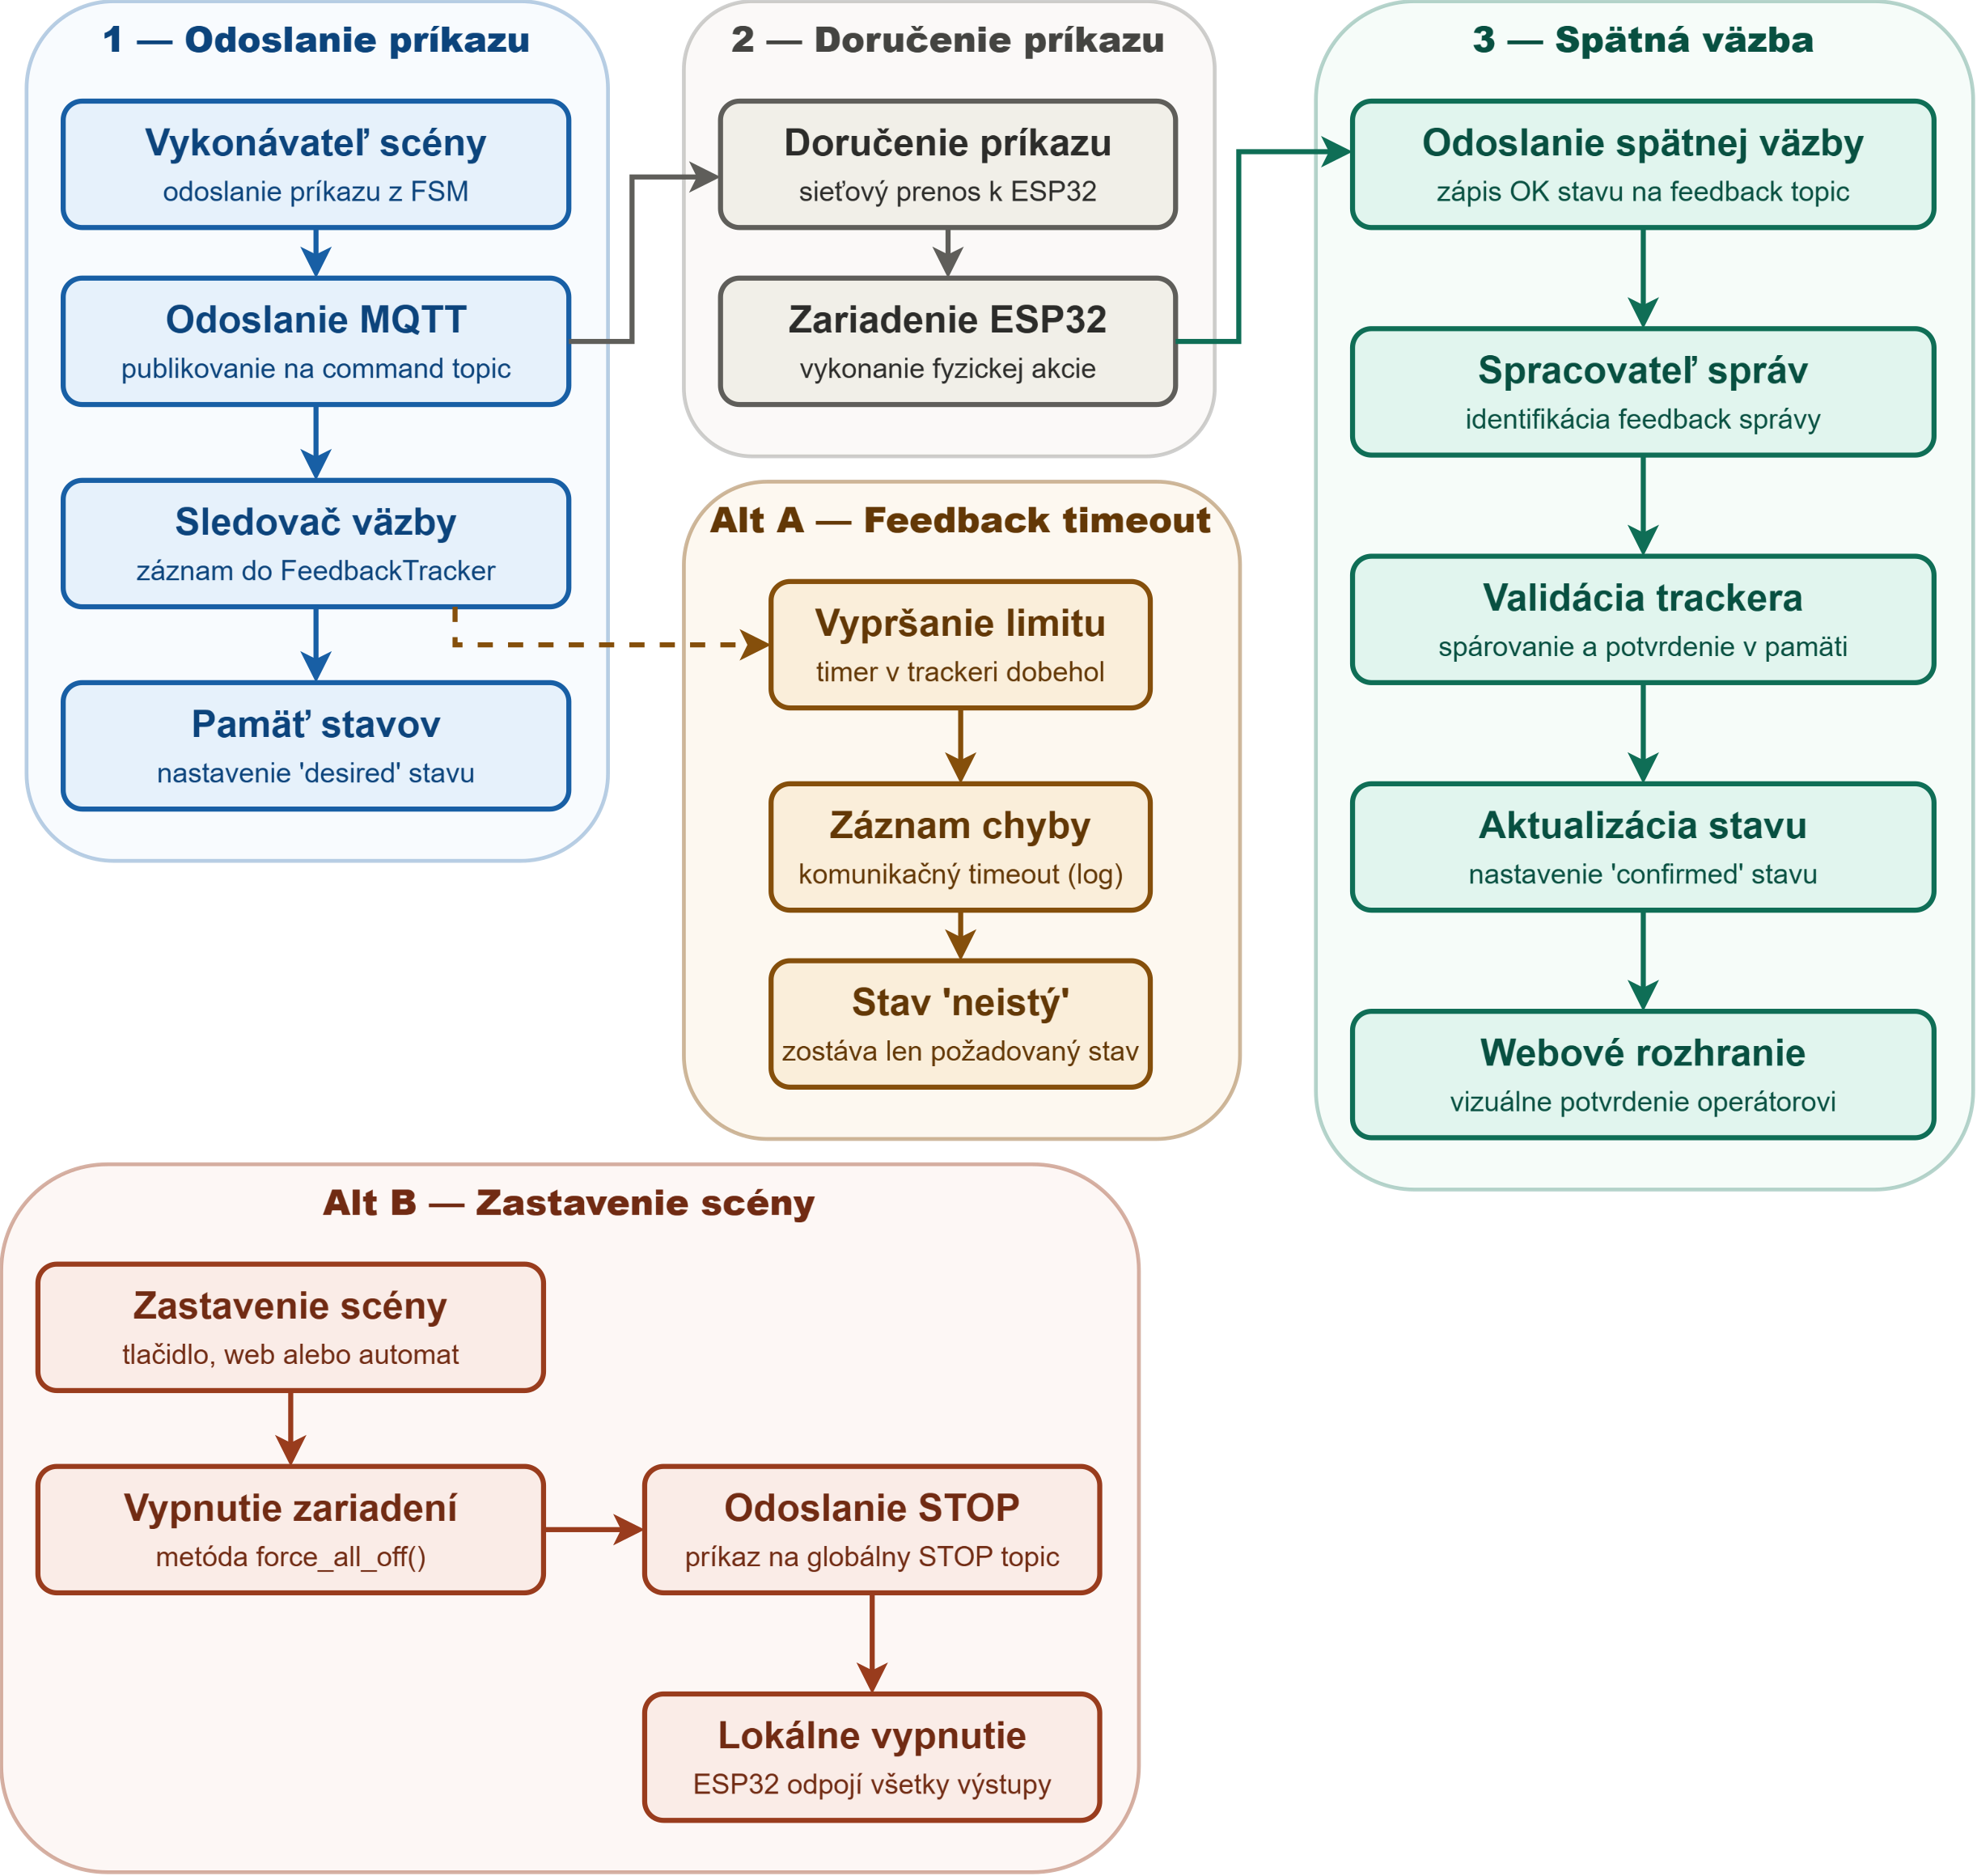
\includegraphics[width=0.95\linewidth]{obr/SW_DIAGRAM_SPECS/5_5_mqtt_sequence_runtime/diagram_5_5_mqtt_sequence_runtime_final.png}
    \caption{Sekvenčný tok MQTT správ pri vykonaní akcie, potvrdení, časovom limite a~zastavení}
    \label{fig:sw_mqtt_flow}
\end{figure}

\subsection{Sledovanie stavu aktuátorov}
\label{SWActuatorStore}

Súčasťou MQTT vrstvy je \textbf{register stavov aktuátorov},
ktorý pre každý príkazový topik udržiava dvojicu:
\textit{desired} (požadovaný stav po odoslaní príkazu)
a~\textit{confirmed} (potvrdený stav po prijatí správy spätnej väzby
\texttt{OK} od uzla). Register oddeľuje okamžitú spätnú väzbu
pre používateľské rozhranie od skutočného hardvérového potvrdenia.
Pri zastavení scény sa nad registrom volá operácia núteného vypnutia,
ktorá nastaví sledované výstupy do bezpečného stavu nezávisle
od oneskorených správ spätnej väzby. Zmeny stavu sú okamžite
propagované do webového dashboardu cez \textbf{WebSocket}.

\section{Mediálna vrstva a~webové rozhranie}
\label{SWMediaWeb}

Mediálna a~webová časť systému pozostáva z~troch samostatných podsystémov:

\begin{itemize}
    \item \textbf{Zvuková vrstva.}
        Kombinuje dva režimy prehrávania: zvukové efekty určené
        na okamžité prehrávanie sa pred štartom scény načítajú
        do pamäte RAM na zníženie latencie,
        zatiaľ čo dlhšie hudobné stopy sú streamované priebežne
        z~disku. Prescan a~preloading prebehnú ešte pred štartom
        stavového automatu.

    \item \textbf{Video vrstva.}
        Je realizovaná prostredníctvom prehrávača \textbf{mpv}
        spusteného v~režime celej obrazovky. Prehrávač je riadený
        cez \textbf{IPC rozhranie} na báze UNIX socketu; počas
        behu sa periodicky kontroluje dostupnosť procesu
        a~odozva ovládacieho kanála.

    \item \textbf{Webové rozhranie.}
        Poskytuje obsluhe prevádzkové funkcie bez zásahu
        do konzoly. Frontend je realizovaný ako \textbf{React} SPA
        a~backend ako \textbf{Flask} služba s~vrstvou
        \textbf{Flask-SocketIO}. Rozhranie zahŕňa spúšťanie
        a~zastavovanie scén, odosielanie príkazov, správu médií
        a~monitorovanie zariadení a~logov. Server priebežne odosiela
        stavové udalosti, takže operátor vidí zmeny bez periodického
        dotazovania zo strany klienta.
        Funkčné členenie dashboardu vychádza z~oddelenia
        serverových udalostí, požiadaviek klienta a~panelov
        používateľského rozhrania (Obr.~\ref{fig:sw_dashboard});
        výsledná hlavná stránka poskytuje operátorovi súhrnný
        prevádzkový pohľad (Obr.~\ref{fig:sw_dashboard_screenshot}).
\end{itemize}

\begin{figure}[htbp]
    \centering
    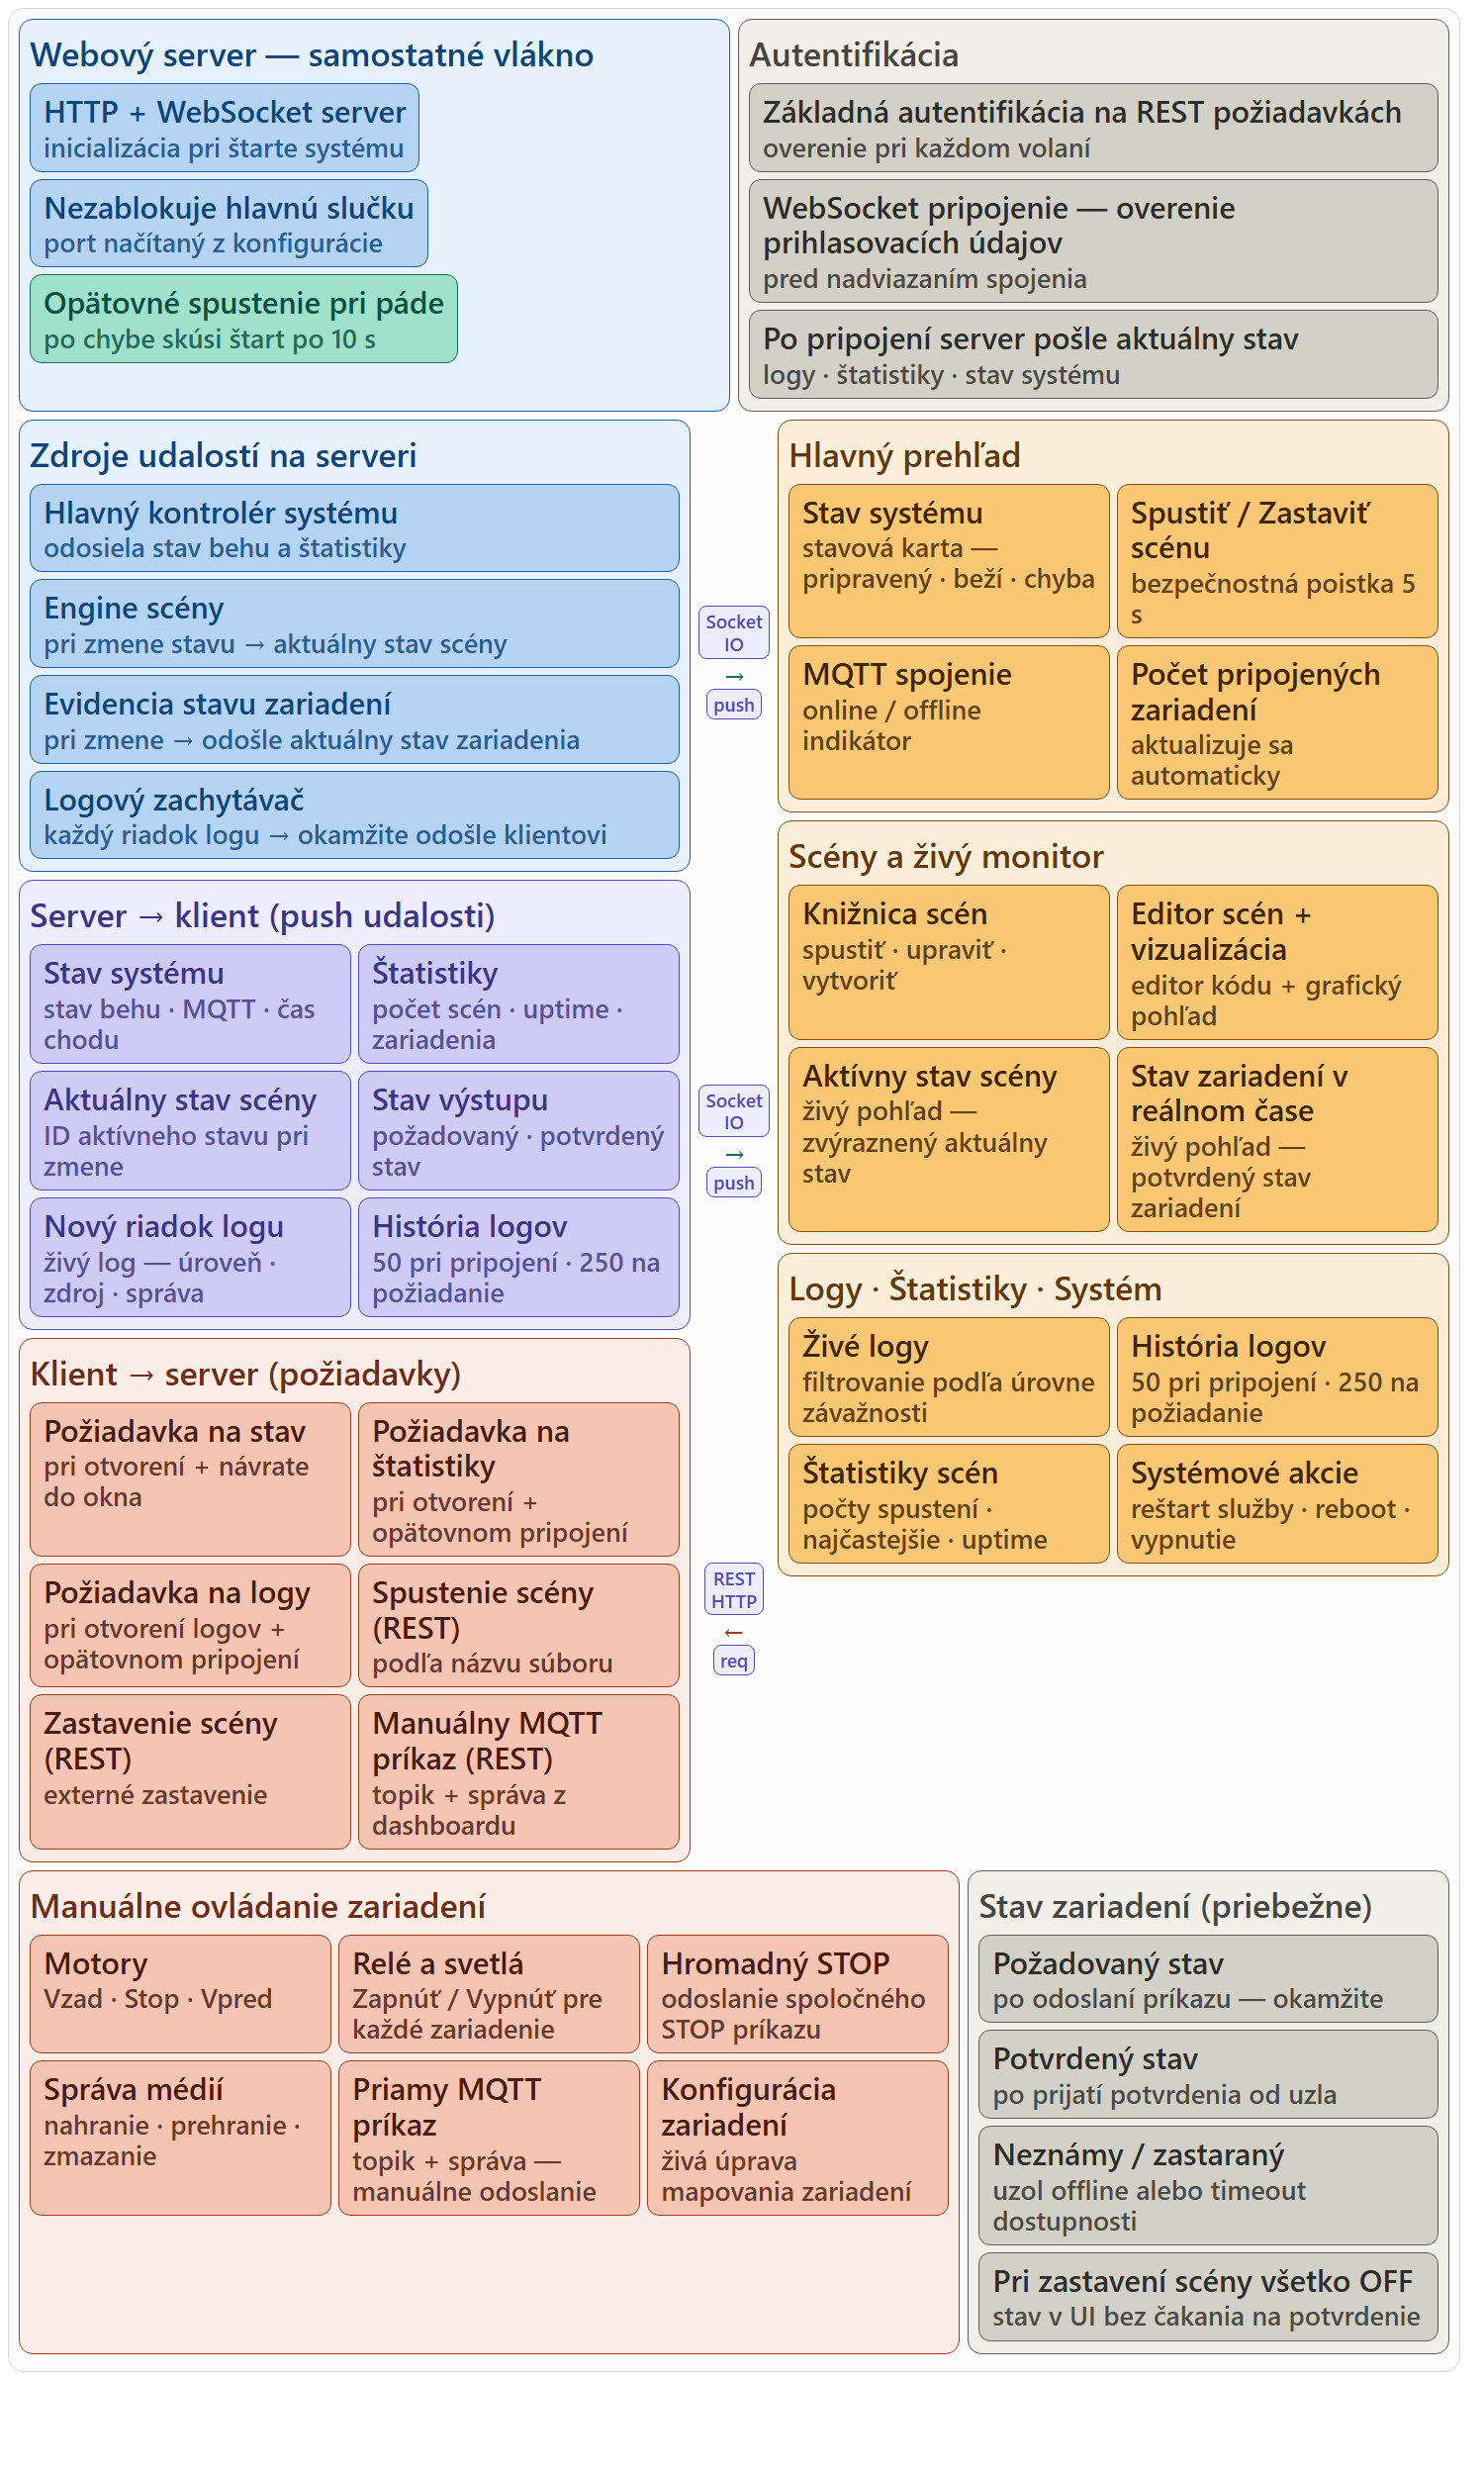
\includegraphics[width=0.92\linewidth]{obr/SW_DIAGRAM_SPECS/5_6_dashboard_functional_view/diagram_5_6_web_dashboard_functional_final.png}
    \caption{Funkčné časti webového dashboardu a~tok udalostí}
    \label{fig:sw_dashboard}
\end{figure}

\begin{figure}[htbp]
    \centering
    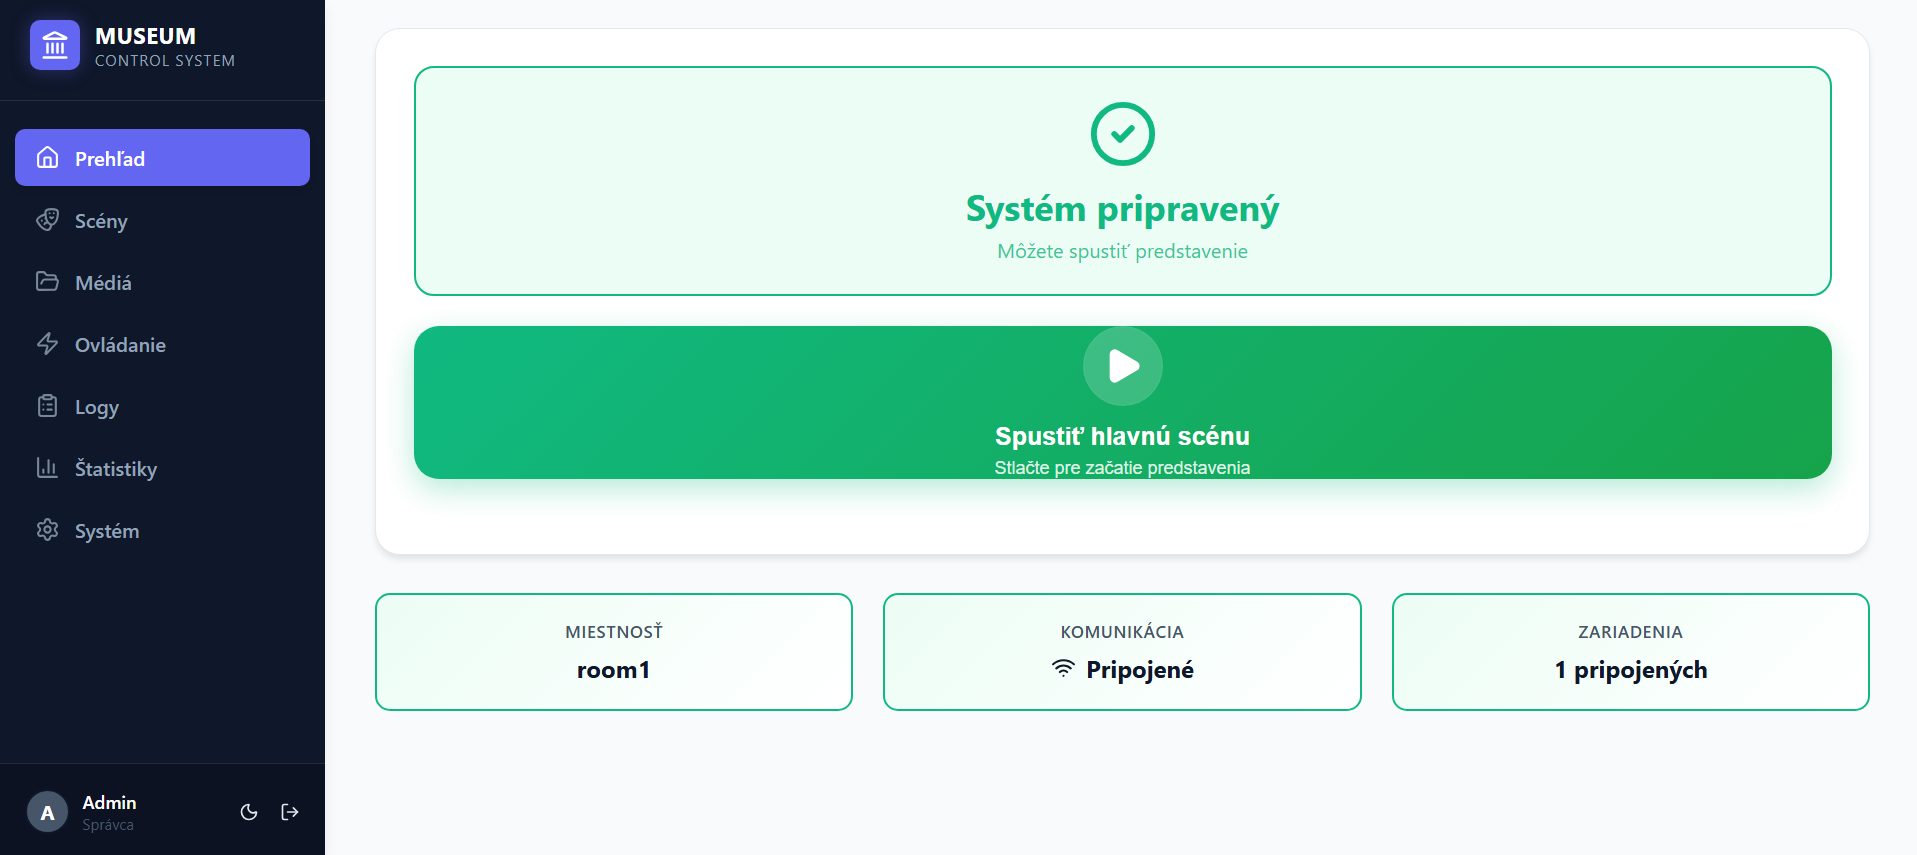
\includegraphics[width=0.95\linewidth]{obr/SW/dashboard_screenshot.png}
    \caption{Hlavná stránka webového dashboardu}
    \label{fig:sw_dashboard_screenshot}
\end{figure}

\section{Firmvér uzlov ESP32}
\label{SWESP32}

Periférna vykonávacia vrstva bola rozdelená na tri firmvérové
varianty pre uzly ESP32. Ich úlohy sa líšia podľa pripojeného
hardvéru, zatiaľ čo sieťová a~servisná časť firmvéru zostáva
vo všetkých prípadoch spoločná.

Firmvér všetkých troch uzlov je napísaný v~jazyku \textbf{C++}
a~bol vytvorený v~prostredí Arduino IDE s~využitím Arduino frameworku
pre mikrokontroléry ESP32.

Spoločná časť firmvéru tvorí servisnú vrstvu, ktorá zabezpečuje
pripojenie k~Wi-Fi a~MQTT, automatické obnovenie spojenia,
periodické stavové hlásenie dostupnosti, LWT správu pre prípad
výpadku, watchdog a~bezdrôtovú aktualizáciu firmvéru. Táto vrstva
zjednocuje správanie uzlov a~špecifická logika sa potom obmedzuje
na lokálnu vstupnú alebo výstupnú úlohu daného zariadenia
(Obr.~\ref{fig:sw_esp_compare}).

\textbf{Tlačidlový uzol} spracúva fyzické stlačenie tlačidla. Vstup
je filtrovaný debouncingom a~dočasným blokovaním opakovaného stlačenia,
aby sa pri jednom fyzickom podnete neposielala rovnaká spúšťacia
správa viackrát za sebou v~krátkom čase. Po potvrdenom stlačení
uzol publikuje spúšťaciu správu scény a~príkazové topiky neodoberá.
Zároveň je pri tlačidle použitý PWM výstup pre LED prstenec, ktorý
slúži na lokálnu stavovú signalizáciu a~potvrdenie stlačenia.

\textbf{Motorický uzol} spracúva príkazy pre dva DC pohony. Firmvér
riadi smer a~rýchlosť pohybu pomocou PWM a~pri zmene smeru zabezpečuje
plynulé zastavenie a~rozbeh motora, aby nevznikali nárazové zmeny
v~mechanike.

\textbf{Reléový uzol} spína výstupy podľa mapovania topik~--~kanál
a~podporuje aj efektové skupiny s~voliteľným automatickým vypnutím.
Uzol tak dokáže lokálne vykonať jednoduché časované akcie bez toho,
aby musel každý krok samostatne riadiť backend.

Bezpečnostné vypnutie pri strate MQTT spojenia, príkaze zastavenia
a~timeoutu nečinnosti je implementované na motorickom a~reléovom
uzle, ktoré zároveň odosielajú spätnú väzbu o~vykonaní príkazu.

\begin{figure}[htbp]
    \centering
    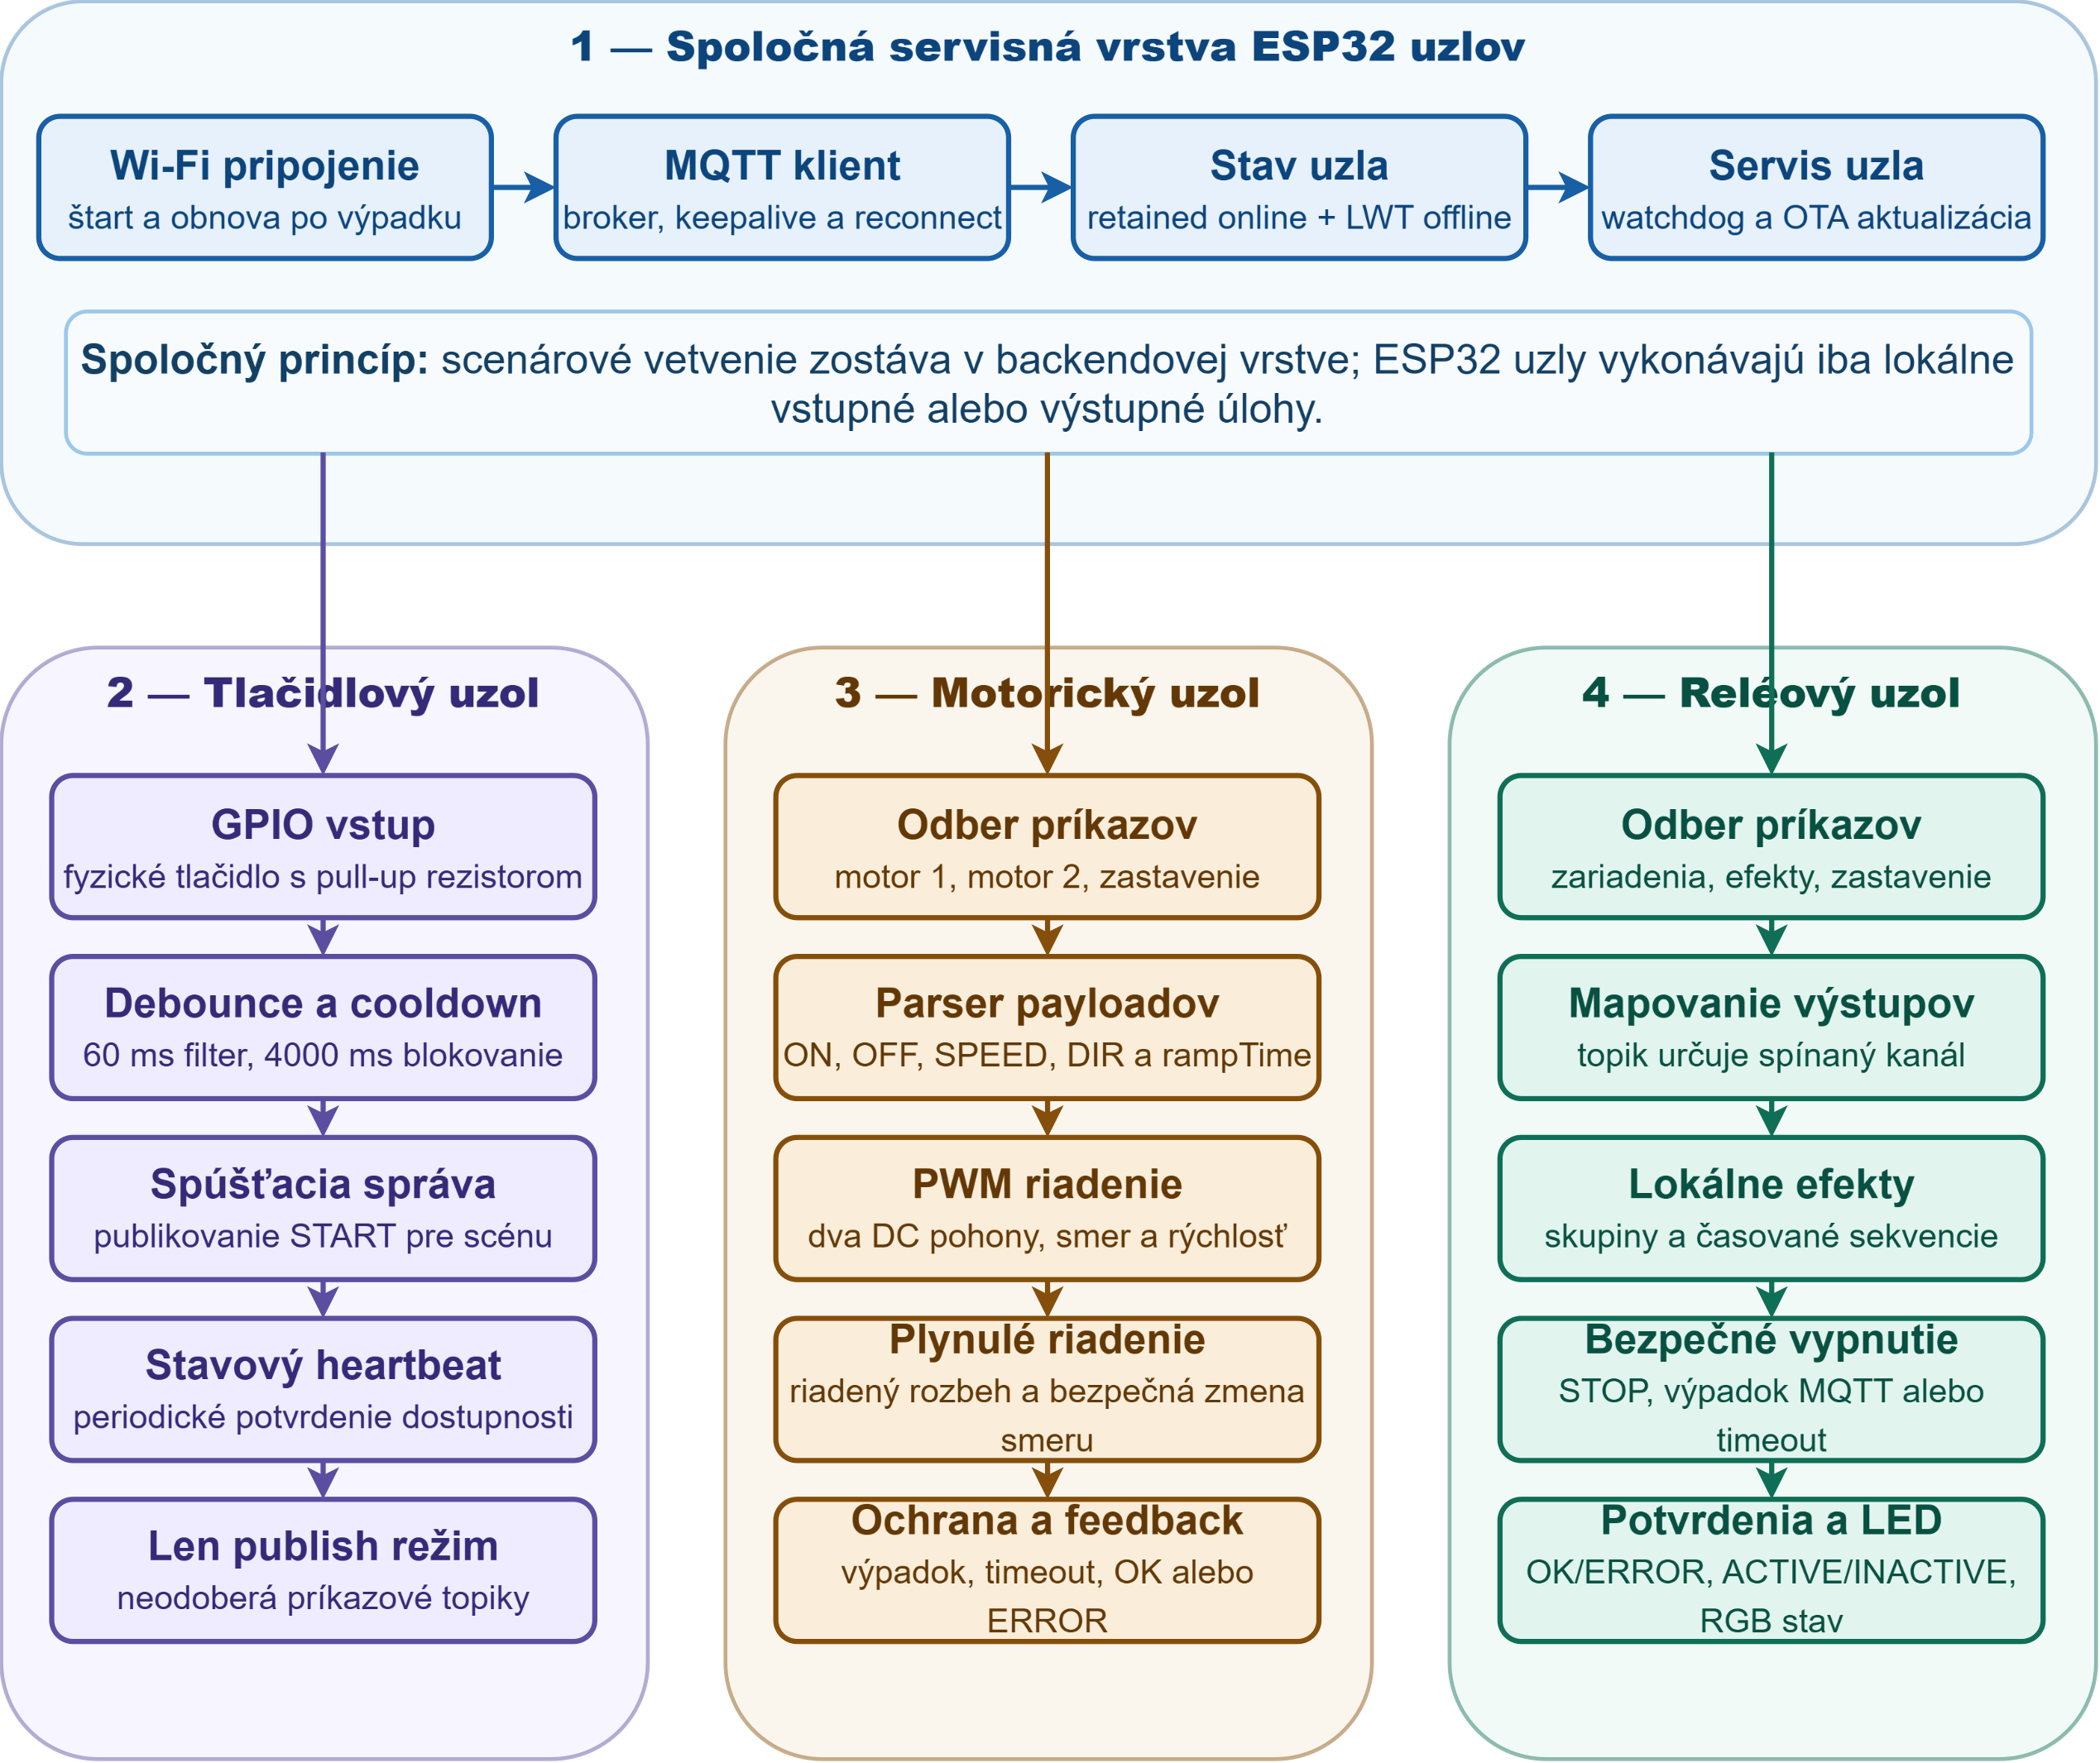
\includegraphics[width=0.95\linewidth]{obr/SW_DIAGRAM_SPECS/5_7_esp32_common_vs_specific/diagram_5_7_esp32_common_vs_specific_final.png}
    \caption{Spoločná infraštruktúra a~špecifická logika uzlov ESP32}
    \label{fig:sw_esp_compare}
\end{figure}

\section{Zhrnutie kapitoly}
\label{SWZhrnutie}

Softvérová implementácia prepája centrálnu orchestráciu na Raspberry~Pi
s~lokálnym vykonávaním akcií na uzloch ESP32. Jadrom riešenia je
\textbf{stavový automat} s~externou \textbf{JSON konfiguráciou} scén,
\textbf{MQTT komunikáciou} so spätnou väzbou a~\textbf{watchdog službou}
pre reštart backendu bez prerušenia aktívnej scény.
Spoľahlivosť a~funkčnosť implementovaného hardvérovo-softvérového reťazca
sú následne overené experimentálne v~kapitole~\ref{ExperimentalneOverenie}.
